\section{Résultats Numériques}

Les résultats de l'étude statistique sont dans les fichiers de type \verb|stats_XX.json|, et sont triés suivant 10 catégories. 

\begin{figure}[!ht]
	\centering
	\begin{subfigure}[b]{0.45\textwidth}
		\begin{description}
			\item[0] \verb|Signal|
			\item[1] \verb|Other higgs->WW*|
			\item[2] \verb|Other higgs|
			\item[5] \verb|2 fermions leptonic|
			\item[6] \verb|2 fermions hadronic|
			\item[8] \verb|4 fermions hadronic|
			\item[9] \verb|4 fermions semileptonic|
			\item[7] \verb|4 fermions leptonic|
		\end{description}
		\label{stats:results:WW}
		\caption{Pour le canaux \WW}
	\end{subfigure}
     \hfill
	\begin{subfigure}[b]{0.45\textwidth}
		\begin{description}
			\item[0] \verb|Signal|
			\item[3] \verb|Other higgs->bb|
			\item[4] \verb|Other higgs|
			\item[5] \verb|2 fermions leptonic|
			\item[6] \verb|2 fermions hadronic|
			\item[8] \verb|4 fermions hadronic|
			\item[9] \verb|4 fermions semileptonic|
			\item[7] \verb|4 fermions leptonic|
		\end{description}
		\caption{Pour le canaux \bb}
		\label{stats:results:bb}
	\end{subfigure}
	\label{stats:results}
	\caption{Les numéros et les noms des différentes catégories d'\analysis pour l'étude statistique}
\end{figure}

Et dans chaque catégorie, plusieurs variables sont calculées \Figure{\ref{stats:results:vrb}}.

\begin{figure}[!ht]
	\centering
	\begin{description}
		\item[\texttt{name}] nom du type de l'évènement, 
				cité dans \Figure{\ref{stats:results}}
		\item[\texttt{stat}] nombre total d'évènement mesuré
		\item[\texttt{sum}] somme des poids de chaque évènement (signal sur bruit)
		
		\item[\texttt{statPreSel}] nombre d'évènement pré-sélectionnés par la BDT
		\item[\texttt{effPreSel}] taux de pré-sélection
		\item[\texttt{sumPreSel}] somme des poids des évènements pré-sélectionnés 
		
		\item[\texttt{effSel}] taux de sélection
		\item[\texttt{sumSel}] somme des poids des évènements sélectionnés
	\end{description}
	\caption{Variables statistiques de chacune des catégories précédentes \Figure{\ref{stats:results}}}
	\label{stats:results:vrb}
\end{figure}

\subsection{Partie \original}

Regardons 2 résultats d'\analysis différents pour \bb, dans le cas d'un signal \Figure{\ref{stats:results:img}} :

\begin{figure}[!ht]
	\centering
	\begin{subfigure}[b]{0.45\textwidth}
		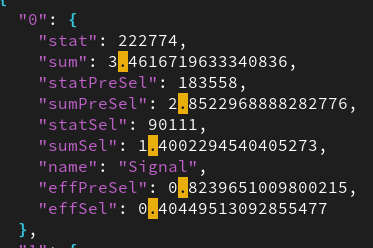
\includegraphics[width=\textwidth]{../img/stats_bb_original_run1_run1.png} 
		\label{stats:results:bb:original:1:1}
		\caption{Canal \bb, branche \original, run 1}
	\end{subfigure}
     \hfill
	\begin{subfigure}[b]{0.45\textwidth}
		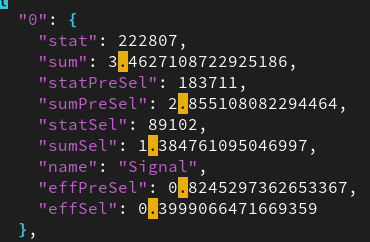
\includegraphics[width=\textwidth]{../img/stats_bb_original_run2_run1.png}
		\caption{Canal \bb, branche \original, run 2}
		\label{stats:results:bb:original:2:1}
	\end{subfigure}
	\label{stats:results:img}
	\caption{Les numéros et les noms des différentes catégories d'\analysis pour l'étude statistique}
\end{figure}

On constate un écart initial sur le nombre d'évènement de moins de 0.01\%, puis une diminution des évènements pré-sélectionnés de 17,6\% pour le \textit{run 1} contre 17,5\% pour le \textit{run 2}. Et une diminution de 59,6\% et 60,0\% pour les évènements sélectionnés par la BDT. 

L'autre constat est qu'on subit une grosse diminution entre les variables \texttt{sum} et \texttt{effSel}, de 88,3\% et 88,5\%, ce qui traduit une baisse importante de luminosité induit par le signal, une fois débarrassée du bruit de fond. Mais une fois encore ces résultats sont cohérents. \\

Donc même si les résultats sont proches, ils ne sont pas identiques puisque la BDT utilise des nombres aléatoires dans sa prise de décision sur le type d'évènement. Mais le programme reste robuste, et que l'utilisation d'une BDT n'est pas une solution idéale puisqu'elle induise une incertitude numérique supplémentaire.